%% == Casio VZ Virtual Instrument =============================================
%%    A virtual replica of the Casio VZ-1/VZ-10M music synthesizer
%% 
%% Matthias Wolff, BTU Cottbus-Sentenberg
%% August 30, 2019
%% DOI 
%%
%% References:
%% [1] 
%%
\documentclass[a4paper]{article}
%
% Packages
\usepackage{amsmath}
\usepackage{amssymb}
\usepackage[dvipsnames]{xcolor}
\usepackage{xspace}
\usepackage{authblk}
\usepackage[capitalize]{cleveref}
\usepackage{url}
\usepackage{tikz}
\usepackage[european]{circuitikz}
\usepackage{subcaption}
\usepackage{booktabs}
%
% Names
%\newcommand{\Ntikz}{TikZ\xspace}
%
% Custom commands
\def\d{\mathrm{d}}
\def\e{\mathrm{e}}
\def\i{\mathrm{i}}
\newcommand\person[1]{\textsc{#1}}
\newcommand{\TT}[1]{\protect\scalebox{0.75}[1.04]{\texttt{#1}}}
\newcommand\WBOX[1]{\vspace*{3pt}{%
  \setlength{\fboxrule}{0.5pt}%
  \setlength{\fboxsep}{3pt}
  
  \noindent\fbox{\begin{minipage}{0.985\textwidth}
  #1
  \end{minipage}}}\vspace*{3pt}
  
}
\newcommand\REMARK[1]{\WBOX{\textbf{Remark: }#1}}
\newcommand\ISSUE[1]{\WBOX{\textbf{Issue: }#1}}
\newcommand{\CORR}[1]{{\color{red!90!RoyalBlue}#1}}
\newcommand{\workOn}{\color{Salmon!80!black}}
\newcommand{\workOff}{\color{black}}
\newcommand{\TODO}[1]{%
  \fboxsep=1pt\fboxrule=1pt\fcolorbox{yellow}{white}{[\textbf{TODO:~}#1]}%
}
\newcommand{\CHECK}[1]{%
  \fboxsep=1pt\fboxrule=1pt\fcolorbox{yellow}{white}{#1}%
}
\def\ML{\text{\smash{\raisebox{-3.5pt}{
\includegraphics{images/matlab}}}\,}}
\def\sOSCsym{\tikz \draw[x=1ex,y=1ex] (0,0) sin (1,2) cos (2,0) sin (3,-2) cos (4,0);}
\def\rOSCsym{\tikz \draw[x=1ex,y=1ex] (0,0) -- (4,4);}
\DeclareMathOperator{\wf}{w}
%
% Settings
% - Page layout
\renewcommand{\floatpagefraction}{.8}
\textheight242mm
\textwidth150mm
\marginparwidth28mm
\topmargin-15mm
\oddsidemargin0mm
\evensidemargin0mm
% - Other
%\setcounter{secnumdepth}{2}

%%%%%%%%%%%%%%%%%%%%%%%%%%%%%%%%%%%%%%%%%%%%%%%%%%%%%%%%%%%%%%%%%%%%%%%%%%%%%%%

\begin{document}
%
\author{Matthias Wolff$^{\text{\sf\,[0000--0002--3895--7313]}}$}
\affil{BTU Cottbus-Senftenberg}
\title{Casio VZ Virtual Instrument:\\
A Replica of the Casio VZ-1/VZ-10M Music Synthesizer}
\maketitle

\bigskip\noindent
See \TT{https://github.com/matthias-wolff/Casio-VZ-virtual-instrument/blob/master/Casio-VZ-virtual-instrument.pdf}
for the latest version of this document.
\begin{center}
  \bigskip\bigskip
  \begin{minipage}{0.9\linewidth}
    \textbf{Abstract}

    \bigskip
In this project I try to rebuild the vintage Casio VZ-1/VZ-10M music synthesizer
in Reaktor 6 \cite{Reaktor6}. The primary goal is a fully functional player
which is compatible with MIDI editor/librarian software like Midi Quest
\cite{MidiQuest12} or the like. My workplan is
\begin{enumerate}   
  \item 
    make some debugging and development tools (waveform validator, envelope
    validator, etc.),
  \item
    reproduce the 8 core waveforms of VZ-1/VZ-10M (1x sine, 5x sawtooth-like
    waveforms created by Casio's Phase Distortion Modulation, 1x white noise, 1x
    pitch-sensitive narrow-band noise),
  \item
    implement the core sound engine (wavetable oscillators, phase and ring
    modulators, VCAs, oscillator circuits),
  \item
    implement control signal generators (amplitude envelope, key following,
    layering, parametric sensitivity characterisitcs, etc.),
  \item
    implement MIDI SysEx control capability, and
  \item
    reproduce the factory voice and operation libraries.
\end{enumerate}
I always strongly disliked the unpleasant---though most
characteristic---aliasing and analog noise of the VZ-1. Hence, I will not
attempt to reproduce this. Insofar, the remake is not intended to be perfect.

As a secondary goal I may want to reproduce the GUI of the original instrument.
This would be a nice-to-have, however not necessarily of much practical use.

  \end{minipage}
  \vfill
  \vfill
\end{center}
\clearpage

\tableofcontents
\clearpage

%%%%%%%%%%%%%%%%%%%%%%%%%%%%%%%%%%%%%%%%%%%%%%%%%%%%%%%%%%%%%%%%%%%%%%%%%%%%%%%

\section{Goals and Prerequisites}
In this project I try to rebuild the vintage Casio VZ-1/VZ-10M music synthesizer
in Reaktor 6 \cite{Reaktor6}. The primary goal is a fully functional player
which is compatible with MIDI editor/librarian software like Midi Quest
\cite{MidiQuest12} or the like. My workplan is
\begin{enumerate}   
  \item 
    make some debugging and development tools (waveform validator, envelope
    validator, etc.),
  \item
    reproduce the 8 core waveforms of VZ-1/VZ-10M (1x sine, 5x sawtooth-like
    waveforms created by Casio's Phase Distortion Modulation, 1x white noise, 1x
    pitch-sensitive narrow-band noise),
  \item
    implement the core sound engine (wavetable oscillators, phase and ring
    modulators, VCAs, oscillator circuits),
  \item
    implement control signal generators (amplitude envelope, key following,
    layering, parametric sensitivity characterisitcs, etc.),
  \item
    implement MIDI SysEx control capability, and
  \item
    reproduce the factory voice and operation libraries.
\end{enumerate}
I always strongly disliked the unpleasant---though most
characteristic---aliasing and analog noise of the VZ-1. Hence, I will not
attempt to reproduce this. Insofar, the remake is not intended to be perfect.

As a secondary goal I may want to reproduce the GUI of the original instrument.
This would be a nice-to-have, however not necessarily of much practical use.

\subsection{The VZ-1/VZ-10M Music Synthesizer}
\TODO{\ldots}

\subsection{The Reaktor 6 Modular DSP Lab}
\TODO{\ldots}
\cite{Reaktor6}

\subsection{The Midi Quest 12 Editor/Librarian Software}
\TODO{\ldots}
\cite{MidiQuest12}

%%%%%%%%%%%%%%%%%%%%%%%%%%%%%%%%%%%%%%%%%%%%%%%%%%%%%%%%%%%%%%%%%%%%%%%%%%%%%%%

\section{Development and Debugging Tools}
\subsection{Waveform Validator}
\TODO{\ldots}

\subsection{Envelope Validator}
\TODO{\ldots}

%%%%%%%%%%%%%%%%%%%%%%%%%%%%%%%%%%%%%%%%%%%%%%%%%%%%%%%%%%%%%%%%%%%%%%%%%%%%%%%

\section{Development and Debugging Tools}

%%%%%%%%%%%%%%%%%%%%%%%%%%%%%%%%%%%%%%%%%%%%%%%%%%%%%%%%%%%%%%%%%%%%%%%%%%%%%%%

\section{Core Sound Engine}
VZ's sound engine is called ``iPD (interactive phase distortion) modular sound
engine'' \cite[p.\,12]{VZ1Manual}. According to Casio, this is an enhanced
version of the phase distortion modulation introduced by the predecessor of the
VZ-1 called CZ-1 \cite[p.\,39]{FS89}. Actually, the VZ synths series seem to
feature wavetable oscillators---with waveforms partly generated by the original
PD synthesis---together with ordinary phase modulation and ring modulation.

\subsection{Theory}
I assume that the reader is familiar with the basics of signal processing.
Introductions can be found in \cite{HW14} and \cite{OS14}.

\subsubsection{Tones, Timbre, Frequency, and Pitch}
\label{sssec:ttfp}
A musical tone is a periodic osciallation of sound pressure. Mathematically, we
express musical tones as real functions
\begin{equation}
  \notag
  x: \mathbb{R}\to \mathbb{R}
\end{equation}
which assign signal values $x(t)\in\mathbb{R}$ to instants of time
$t\in\mathbb{R}$ measured in seconds. We will call such functions ``signals''.
As a musical tone is periodic, the corresponding signal must be periodic as
well. Mathematically, we express this by the condition
\begin{equation}
  \label{eqn:periodic}
  x(t+nT) = x(t)
  \qquad\text{with }n\in\mathbb{Z},
\end{equation}
where $T$, measured in seconds, is called the cycle duration.
\cref{eqn:periodic} simply means, that the signal values repeate after an
integer number of cylces ist completed. The reciprocal of the cycle duration is
called tone or fundamental frequency
\begin{equation}
  \notag
  f = \frac{1}{T}.
\end{equation}
Frequencies are measured in Hertz (Hz).

The most basic musical tone is a pure tone. Its mathematical representation as a
signal is
\begin{equation}
  \label{eqn:MtCosine}
  x_{\cos}(t) = a_1\cos(2\pi f t+\varphi_1),
\end{equation}
where $a_1$ denotes the amplitude which is connected to the perceived loudness,
$f$ denotes the tone frequency which is connected to the perceived pitch, and
$\varphi_1$ denotes a phase offset which does not directly relate to
perception. \cref{fig:MtCosine} shows the plot of a cosine signal. As the cosine
function is periodic, $\cos(\alpha+2\pi n)=\cos(\alpha)$, so is the cosine
signal. The cycle duration of the cosine signal is $T=1/f$. Note, that the
mathematical concept of signals abstracts from sound pressure oscillations. We
can also use it for oscillations of other physical quantities like voltages and
even for any digital representations of such quantities.

As $\cos(\alpha) = \sin(\alpha+\pi/2)$, pure tones can also be expressed by the
sine function
\begin{equation}
  \notag
  %\label{eqn:MtSine}
  x_{\cos}(t) = a_1\sin\left(2\pi f t+\varphi_1+\frac{\pi}{2}\right)\!.
\end{equation}
Cosine and sine tones are indistinguishable to the human ear. Hence, both are
commonly referred to as ``sine'' tones.

General musical tones are mixtures of pure tones. We express them mathematically
as a sum of cosine tones
\begin{equation}
  \label{eqn:MtPeriodic}
  x(t) 
  = \sum\limits_{n=1}^\infty a_n\cos\!\big(2\pi nft+\varphi_n)
\end{equation}
The summand with $n=1$ describes the fundamental tone, the summands with $n>1$
describe so called overtones or partials. The frequencies of all overtones are
integer multiples $n\cdot f$ of the tone frequency $f$. General muscial tones
according to \cref{eqn:MtPeriodic} are still periodic with a cycle duration of
$T=1/f$. The fundamental tone and all overtones are characterized by individual
amplitudes $a_n$ and phase offsets $\varphi_n$. The amplitude-phase tuples
$(a_n,\varphi_n)$ are called (real) \person{Fourier} coefficients and
\cref{eqn:MtPeriodic} is called \person{Fourier} series (see, e.g.,
\cite[p.\,102--113]{HW14}).\footnote{Actually, the real \person{Fourier} series
contains a further summand, $a_0$, allowing for a DC offset which we
deliberately exclude here as such offsets are undesirable for musical tones.}
The perceived timbre of a musical tone is mainly connected to the sequence
$(a_n)$ of amplitudes. The sequence of phase offsets $(\varphi_n)$ is
perceptually much less relevant than the ampltitudes. \cref{fig:Mt3Cosines}
shows an example of a muscial tone composed by the mixture of three pure tones.

Even more complex tones comprise aperiodic components (noise) and varying
timbre, i.e. \person{Fourier} coefficients, over time.
%
\begin{figure*}[h]
  \centering
  \begin{subfigure}[t]{0.5\textwidth}
    \centering
    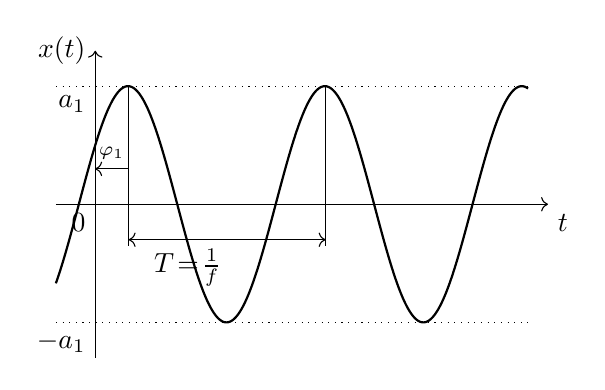
\begin{tikzpicture}[x=2.5cm, y=1.5cm]
      \draw[thin,->] (-0.2,0) -- (2.3,0) node[anchor=north west] {$t$};
      \draw[thin,->] (0,-1.3) -- (0,1.3) node[anchor=east] {$x(t)$};
      \node[anchor=north east] at (0,0) {$0$};
      \draw[thin,dotted] (-0.2, 1) -- (2.2, 1); \node[anchor=north east] at (0, 1) {$a_1$};
      \draw[thin,dotted] (-0.2,-1) -- (2.2,-1); \node[anchor=north east] at (0,-1) {$-a_1$};
      \draw[thick,smooth,samples=500,domain=-0.2:2.2,variable=\x] 
        plot ({\x},{cos(360*\x-60)});
      \draw[thin]     (0.17, 1   ) -- (0.17,-0.35);
      \draw[thin]     (1.17, 1   ) -- (1.17,-0.35);
      \draw[thin,<->] (0.17,-0.3 ) -- (1.17,-0.3 );
      \draw[thin, ->] (0.17, 0.3 ) -- (0   , 0.3 );
      \node[anchor=north west] at (0.25,-0.3) {$T\!=\!\frac{1}{f}$};
      \node[anchor=south] at (0.083,0.3) {$\scriptstyle\varphi_1$};
    \end{tikzpicture}
    \caption{A cosine tone\newline
      $x_{\cos}(t)=a_1\cos(2\pi f t+\varphi_1)$
      \label{fig:MtCosine}}
  \end{subfigure}~
  \begin{subfigure}[t]{0.5\textwidth}
    \centering
    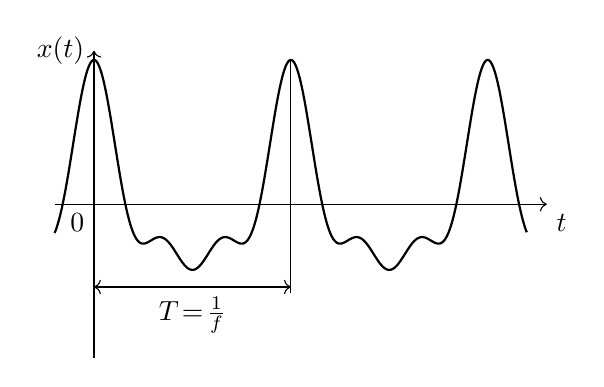
\begin{tikzpicture}[x=2.5cm, y=1.5cm]
      \draw[thin,->] (-0.2,0) -- (2.3,0) node[anchor=north west] {$t$};
      \draw[thin,->] (0,-1.3) -- (0,1.3) node[anchor=east] {$x(t)$};
      \node[anchor=north east] at (0,0) {$0$};
      \draw[thick,smooth,samples=500,domain=-0.2:2.2,variable=\x] 
        plot ({\x},{2/3*(cos(360*\x) + 1/2*cos(2*360*\x) + 1/3*cos(3*360*\x))});
      \draw[thin]     (1, 1.22) -- (1,-0.75);
      \draw[thin,<->] (0,-0.7 ) -- (1,-0.7 );
      \node[anchor=north] at (0.5,-0.7) {$T\!=\!\frac{1}{f}$};
    \end{tikzpicture}
    \caption{A musical tone composed of three cosines \newline
      $x(t)=\frac{2}{3}\sum\nolimits_{n=1}^2 \frac{1}{n}\cos(2\pi n f t)$
      \label{fig:Mt3Cosines}}
  \end{subfigure}
  \caption{Examples for basic musical tones. The tone frequency---measured in
  Hertz---is denoted by $f$. We denote time by $t$ and the duration of one cycle
  by $T$. Both are measured in seconds. The argument of the cosine functions is
  called phase angle $\varphi$. One cycle corresponds to a phase difference of
  $\Delta\varphi = 2\pi$.}
\end{figure*}

Human perception of sound frequency is nearly logarithmic. Therefore, Western 
music theory commonly uses the pitch 
\begin{equation}
  \label{eqn:f2p}
  p = 69 + 12\,\log_2\!\left(\dfrac{f}{440\,\text{Hz}}\right)
  \qquad\qquad\text{\ML \TT{p=vVZtools.f2p(f)}}
\end{equation}
measured in semitones rather than frequencies. The value of $440\,\text{Hz}$ in
the denominator is the concert pitch. The offset of $69$ makes the pitch
computed by \cref{eqn:f2p} compatible with a MIDI frequency data value.
According to the MIDI \CHECK{tuning} standard \TODO{\cite{}}, $p$ takes values
from the interval $0.00\leq p\leq 127.99$ with the integer part corresponding to
a note number and the decimal fraction, with two digits precision, to a detune.
MIDI note number $p=0$ stands for C$_{-1}$, $p=69$ for the concert pitch A$_4$,
and $p=127$ stands for B$_9$.

Solving \cref{eqn:f2p} for $f$, we obtain a formula for converting pitch to
frequency:
\begin{equation}
  \label{eqn:p2f}
  f = 2^{\frac{p-69}{12}}\cdot 440\,\text{Hz}
  \qquad\qquad\text{\ML \TT{f=vVZtools.p2f(p)}}.
\end{equation}

\subsubsection{Oscillators and Waveforms}
\label{sssec:oscWf}
The basic building blocks of music synthesizers are oscillators. An oscillator
is an apparatus, hardware or software, which produces a signal $x(t)$ depending 
on a single frequency $f$. As circuit symbol for an oscillator we will use
\begin{center}
  \begin{circuitikz}%[blocks/scale=0.8] % ->ERROR! WHY?
    \draw (0,0) node[twoportshape, t=\sOSCsym](osc) {};
    \draw (osc.east) to[short,-o] ++(0.5,0) node[anchor=west] {$x(t)$.};
    \draw (osc.north) to [short] ++(0,0.5) node[anchor=south] {$f$};
    \draw (osc.north) node[inputarrow,,rotate=-90] {};
  \end{circuitikz}
\end{center}
In larger circuit diagrams we will omit the frequency input at the top for
legibility.

In software synthesizers, the most basic oscillator type is a so called ramp 
oscillator. A ramp oscillator generates the ramp signal
\begin{equation}
  \notag
  %\label{eqn:rampSig}
  r(t) = ft,
\end{equation}
where $t$ denotes time and $f$ a frequency.\footnote{The term ``oscillator'' is
somewhat misleading here as a ramp signal does not oscillate. Yet, that name
is commonly used.} The circuit symbol and output signal look as follows
\begin{center}
  \hfill
  \raisebox{0.75cm}{
    \begin{circuitikz}[scale=1]
      \draw (0,0) node[twoportshape, t=\rOSCsym](osc) {};
      \draw (osc.east) to[short,-o] ++(0.5,0) node[anchor=west] {$r(t)$};
      \draw (osc.north) to [short] ++(0,0.5) node[anchor=south] {$f$};
      \draw (osc.north) node[inputarrow,rotate=-90] {};
    \end{circuitikz}
  }
  \hfill
  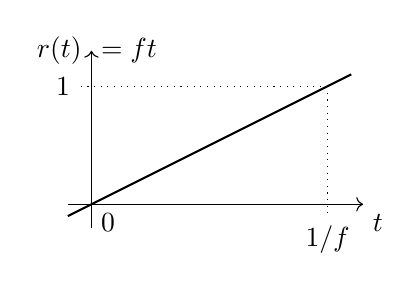
\begin{tikzpicture}[x=1.5cm, y=1.5cm]
    \draw[thin,->] (-0.2,0) -- (2.3,0) node[anchor=north west] {$t$};
    \draw[thin,->] (0,-0.2) -- (0,1.3) node[anchor=east] {$r(t)$};
    \node[anchor=west] at (0,1.3) {$=ft$};
    \node[anchor=north west] at (0,0) {$0$};
    \draw[thin,dotted] (2,1) -- (2,-0.1) node[anchor=north] {$1/f$};
    \draw[thin,dotted] (2,1) -- (-0.1,1) node[anchor=east] {$1$};
    \draw[thick] (-0.2,-0.1) -- (2.2,1.1);
  \end{tikzpicture}
  \hspace*{20pt}
\end{center}
Amplifying the output of a ramp oscillator by a gain factor of $2\pi$ and
feeding the result into a cosine function, we obtain an oscillator circuit for a
pure cosine tone with amplitude $1$ and without phase offset:
\begin{center}
  \hfill
  \raisebox{1.45cm}{
    \begin{circuitikz}
      \draw (0,0) node[twoportshape, t=\rOSCsym](osc) {};
      \draw (osc.north) to [short] ++(0,0.5) node[anchor=south] {$f$};
      \draw (osc.north) node[inputarrow,rotate=-90] {};
      \draw (osc.east) 
        to[short]            ++(0.25,0) 
        to[amp,t=$2\pi$]     ++(1.50,0)
        to[twoport,t=$\cos$] ++(1.50,0)
        to[short,-o]         ++(0.25,0) 
        node[anchor=west] {$x(t)$};
    \end{circuitikz}
  }
  \hfill
  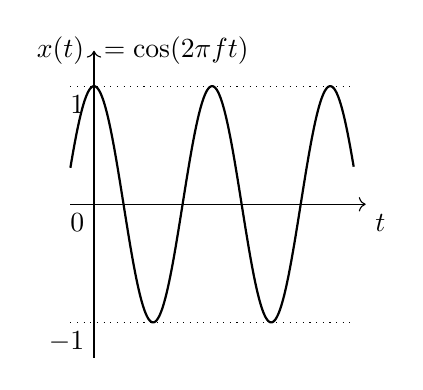
\begin{tikzpicture}[x=1.5cm, y=1.5cm]
    \draw[thin,->] (-0.2,0) -- (2.3,0) node[anchor=north west] {$t$};
    \draw[thin,->] (0,-1.3) -- (0,1.3) node[anchor=east] {$x(t)$};
    \node[anchor=west] at (0,1.3) {$=\cos(2\pi ft)$};
    \node[anchor=north east] at (0,0) {$0$};
    \draw[thin,dotted] (-0.2, 1) -- (2.2, 1); \node[anchor=north east] at (0, 1) {$1$};
    \draw[thin,dotted] (-0.2,-1) -- (2.2,-1); \node[anchor=north east] at (0,-1) {$-1$};
    \draw[thick,smooth,samples=500,domain=-0.2:2.2,variable=\x] 
      plot ({\x},{cos(360*\x)});
  \end{tikzpicture}
  \hspace*{20pt}
\end{center}
Adding anothor amplifier at the output and a phase offset at the input of the
cosine function yields an oscillator circuit for pure tone according to
\cref{eqn:MtCosine}:
\begin{center}
  \hfill
  \raisebox{1.45cm}{
    \begin{circuitikz}
      \draw (0,0) node[twoportshape, t=\rOSCsym](osc) {};
      \draw (osc.north) to [short] ++(0,0.5) node[anchor=south] {$f$};
      \draw (osc.north) node[inputarrow,rotate=-90] {};
      \draw (2.75,0) 
        node[adder,scale=0.66](add){}
        (add.west) node[inputarrow]{}
        (add.north) node[inputarrow,rotate=-90] {};
      \draw (osc.east) 
        to[short]            ++(0.25,0) 
        to[amp,t=$2\pi$]     ++(1.50,0)
        to[short]            (add.west)
        (add.east) 
        to[twoport,t=$\cos$] ++(2,0)
        to[amp,t=$a_1$]      ++(1,0)
        to[short,-o]         ++(0.5,0) 
        node[anchor=west] {$x(t)$};
      \draw (add.north) to [short] ++(0,0.66) node[anchor=south] {$\varphi_1$};
    \end{circuitikz}
  }
  \hfill
  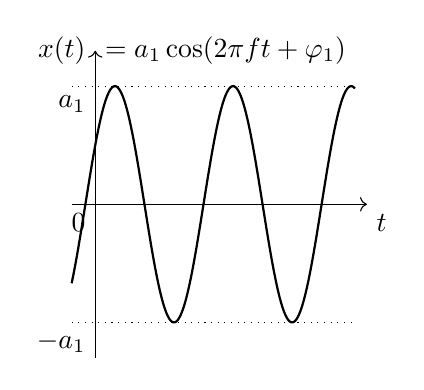
\begin{tikzpicture}[x=1.5cm, y=1.5cm]
    \draw[thin,->] (-0.2,0) -- (2.3,0) node[anchor=north west] {$t$};
    \draw[thin,->] (0,-1.3) -- (0,1.3) node[anchor=east] {$x(t)$};
    \node[anchor=west] at (0,1.3) {$=a_1\cos(2\pi ft+\varphi_1)$};
    \node[anchor=north east] at (0,0) {$0$};
    \draw[thin,dotted] (-0.2, 1) -- (2.2, 1); \node[anchor=north east] at (0, 1) {$a_1$};
    \draw[thin,dotted] (-0.2,-1) -- (2.2,-1); \node[anchor=north east] at (0,-1) {$-a_1$};
    \draw[thick,smooth,samples=500,domain=-0.2:2.2,variable=\x] 
      plot ({\x},{cos(360*\x-60)});
  \end{tikzpicture}
  \hspace*{20pt}
\end{center}
In order to add overtones according to \cref{eqn:MtPeriodic}, we simply mix the
outputs of $N$ cosine oscillators running at frequencies $n\cdot f$ with $1\leq
n\leq N$ as follows:
\begin{center}
  \hfill
  \raisebox{-1cm}{
    \begin{circuitikz}[scale=0.9, transform shape]
      %% Middle branch
      \draw (0,0) node[twoportshape, t=\rOSCsym](osc) {};
      \draw (osc.north) to [short] ++(0,0.5) node[anchor=south] {$f$}; \draw (osc.north) node[inputarrow,rotate=-90] {};
      \draw (osc.east) to [amp,t=$2\pi$] (2.25,0) to [short,-*] (2.25,0);
      \draw (3,0) node[mixer,scale=0.66](mix2){};
      \draw (2.25,0) to (mix2.west) node[inputarrow]{};
      \draw (mix2.north) to [short] ++(0,0.33) node[anchor=south] {$2$}; \draw (mix2.north) node[inputarrow,rotate=-90] {};
      \draw (4,0) node[adder,scale=0.66](add2){};
      \draw (mix2.east) to (add2.west) node[inputarrow]{};
      \draw (add2.north) to [short] ++(0,0.33) node[anchor=south] {$\varphi_2$}; \draw (add2.north) node[inputarrow,rotate=-90] {};
      \draw (7.7,0) node[adder,scale=0.66](addE){};
      \draw (add2.east) 
        to [twoport,t=$\cos$] (6,0)
        to [amp,t=$a_2$]      (7,0)
        to (addE.west)
        (addE.west) node[inputarrow]{};
      \draw (addE.east) to[short,-o] ++(0.5,0) node[anchor=west] {$x(t)$};
      %% Top branch
      \draw (4,1.5) node[adder,scale=0.66](add1){}; \draw (add1.west) node[inputarrow] {};
      \draw (2.25,0) -- (2.25,1.5) -- (add1.west);
      \draw (add1.north) to [short] ++(0,0.33) node[anchor=south] {$\varphi_1$}; \draw (add1.north) node[inputarrow,rotate=-90] {};
      \draw (add1.east) 
        to [twoport,t=$\cos$] (6,1.5)
        to [amp,t=$a_1$]      (7,1.5)
        to [short]            (7.7,1.5)
        to [short] (addE.north) node[inputarrow,rotate=-90] {};
      %% Bottom branch
      \draw (3,-2.5) node[mixer,scale=0.66](mixN){};
      \draw (mixN.north) to [short] ++(0,0.33) node[anchor=south] {$N$}; \draw (mixN.north) node[inputarrow,rotate=-90] {};
      \draw (4,-2.5) node[adder,scale=0.66](addN){};
      \draw (addN.north) to [short] ++(0,0.33) node[anchor=south] {$\varphi_N$}; \draw (addN.north) node[inputarrow,rotate=-90] {};
      \draw (2.25,0) -- (2.25,-2.5) -- (mixN.west);
      \draw (mixN.east) -- (addN.west) node[inputarrow] {};
      \draw (addN.east) 
        to [twoport,t=$\cos$] (6,-2.5)
        to [amp,t=$a_N$]      (7,-2.5)
        to [short]            (7.7,-2.5)
        to [short] (addE.south) node[inputarrow,rotate=90] {};
      %% Ellipses
      \node at(3,-0.9) {$\vdots$};
      \node at(4,-0.9) {$\vdots$};
      \node at(5.15,-0.9) {$\vdots$};
      \node at(6.4,-0.9) {$\vdots$};
    \end{circuitikz}
  }
  \hfill
  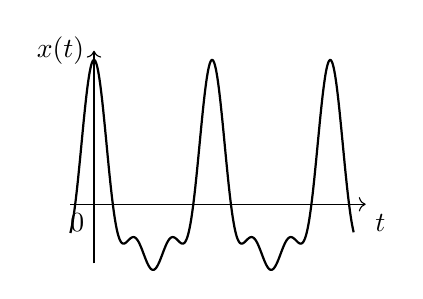
\begin{tikzpicture}[x=1.5cm, y=1.5cm]
      \draw[thin,->] (-0.2,0) -- (2.3,0) node[anchor=north west] {$t$};
      \draw[thin,->] (0,-0.5) -- (0,1.3) node[anchor=east] {$x(t)$};
      \node[anchor=north east] at (0,0) {$0$};
      \draw[thick,smooth,samples=500,domain=-0.2:2.2,variable=\x]
        plot ({\x},{2/3*(cos(360*\x) + 1/2*cos(2*360*\x) + 1/3*cos(3*360*\x))});
  \end{tikzpicture}
  \hspace*{20pt}
\end{center}
Such an osciallator circuit is called a ``sinusoidal oscillator''. Its sound
synthesis paradigm is, for abvious reasons, called ``additive''. Sinusoidal
oscillators are a direct realization of the \person{Fourier} serial according to
\cref{eqn:MtPeriodic} truncated to $N$ terms. However, the circuit is quite
intricate. Therefore, we simplify things by introducing the concept of
waveforms. A waveform is a function
\begin{equation}
  \notag
  %\label{eqn:waveform}
  \wf: \mathbb{R}\to[-1,1],
  \quad x=\wf(\alpha)
\end{equation}
which takes an angle $\alpha$ as argument and which satisfies the following 
conditions:
\begin{alignat}{2}
  %\notag
  \label{eqn:waveformCond1}
  \wf(\alpha+2\pi n)=\wf(\alpha) 
  & \qquad\text{$\wf$ is periodic with a cycle length of $2\pi$,}
\\
  %\notag
  \label{eqn:waveformCond2}
  -1\leq\wf(\alpha)\leq 1
  & \qquad\text{$\wf$ takes values from the interval $[-1,1]$,}
\\
  %\notag
  \label{eqn:waveformCond3}
  \max\limits_{\alpha\in[0,2\pi]}\big(|\wf(\alpha)|\big) = 1
  & \qquad\text{the amplitude of $\wf$ is $1$, and}
\\
  %\notag
  \label{eqn:waveformCond4}
  \int\limits_{0}^{2\pi}\wf(\alpha)\,\d\alpha = 0
  & \qquad\text{$\wf$ has no DC offset.}
\end{alignat}
Clearly, the sine and cosine functions are waveforms by this definition.
A general formula for arbitrary waveforms can be derived from the definition of
musical tones according to \cref{eqn:MtPeriodic}. We set $\alpha = 2\pi ft$
and obtain
\begin{equation}
  \label{eqn:waveformFS}
  \wf(\alpha) = \sum\limits_{n=1}^\infty a_n\cos(n\alpha+\varphi_n).
\end{equation}
The periodicity and DC conditions (\ref{eqn:waveformCond1},
\ref{eqn:waveformCond4}) are implied by \cref{eqn:waveformFS}.
In order to fulfill the amplitude conditions (\ref{eqn:waveformCond2},
\ref{eqn:waveformCond3}), the \person{Fourier} coefficients $a_n$ and
$\varphi_n$ must meet certain criteria which we will not discuss in detail.
\cref{tab:waveforms} shows some examples of typical waveforms used in music
synthesizers.
%
\begin{table}
\workOn
\centering
\begin{tabular}{lll}\toprule
  Name & Waveform & \person{Fourier} coefficients
\\\midrule
  Sine & \TODO{\ldots}
\\
  Rectangle & \TODO{\ldots}
\\
  Triangle & \TODO{\ldots}
\\
  Sawtooth & \TODO{\ldots}
\\\bottomrule
\end{tabular}
\caption{Examples of typical waveforms used in music synthesizers}
\label{tab:waveforms}
\workOff
\end{table}

The circuit diagram of waveform oscillator producing arbitrary musical tones
is
\begin{center}
  \begin{circuitikz}
    \draw (0,0) node[twoportshape, t=\rOSCsym](osc) {};
    \draw (osc.north) to [short] ++(0,0.5) node[anchor=south] {$f$};
    \draw (osc.north) node[inputarrow,rotate=-90] {};
    \draw (3,0) node[twoportshape, t=$\wf$](wf) {};
    \draw (wf.north) to [short] ++(0,0.5) node[anchor=south] {$\big((a_n,\varphi_n)\big)$};
    \draw (wf.north) node[inputarrow,rotate=-90] {};
    \draw (osc.east) 
      to[short]        ++(0.25,0) 
      to[amp,t=$2\pi$] (wf.west)
      (wf.east)
      to[short,-o]     ++(0.50,0) 
      node[anchor=west] {$x(t) = \wf(2\pi ft)$.}
    ;
  \end{circuitikz}
\end{center}
As explained in \cref{sssec:ttfp}, the timbre of the generated tone can be
adjusted by the choice of \person{Fourier} coefficients $\big((a_n, \varphi_n)
\big)$.

\TODO{excursus to samplers?}

\subsubsection{Amplitude and Ring Modulation}
\label{sssec:AMRM}
By the term ``modulation'' we denote techniques of manipulating properties of
a so called carrier signal $x_C(t)$ by a modulating signal $x_M(t)$. Amplitude 
modulation refers to modifiying the carrier's amplitude as follows:
\begin{equation}
  \label{eqn:AM}
  \begin{circuitikz}[baseline=-1ex]
    \draw
      node[anchor=east] at (0, 0) {$x_M(t)$}
      node[anchor=east] at (0,-1) {$x_C(t)$}
      (2.25, 0)   node[adder,scale=0.66](add){}
      (3.25,-1)   node[mixer,scale=0.66](mlt){} 
      (add.west)  node[inputarrow] {}
      (add.north) node[inputarrow,rotate=-90] {}
      (add.north) to [short] ++(0,0.5) node[anchor=south] {$a_C$}
      (mlt.west)  node[inputarrow] {}
      (mlt.north) node[inputarrow,rotate=-90] {}
      (0,0) 
      to[short,o-]    ++(0.25,0)
      to[amp,t=$a_M$] (add.west)
      (add.east)
      to[short] (3.25,0)
      to[short] (mlt.north)
      (0,-1)
      to[short,o-] (mlt.west)
      (mlt.east)
      to[short,-o] ++(0.5,0)
      node[anchor=west] {$x_{\text{AM}}(t) = \big(a_C+a_M\,x_M(t)\big)\cdot x_C(t)$.}
    ;
  \end{circuitikz}
\end{equation}

Ring modulation is a related concept. Here, the gain factor $a_C$ of
the carrier is zero and the gain factor $a_M$ of the modulating signal is one
which yields
\begin{equation}
  \label{eqn:RM}
  \begin{circuitikz}[baseline=-4ex]
    \draw
      node[anchor=east] at (0, 0) {$x_M(t)$}
      node[anchor=east] at (0,-1) {$x_C(t)$}
      (1,-1)      node[mixer,scale=0.66](mlt){} 
      (mlt.west)  node[inputarrow] {}
      (mlt.north) node[inputarrow,rotate=-90] {}
      (0,0) 
      to[short,o-] ++(1,0)
      to[short]    (mlt.north)
      (0,-1)
      to[short,o-] (mlt.west)
      (mlt.east)
      to[short,-o] ++(0.5,0)
      node[anchor=west] {$x_{\text{RM}}(t) = x_M(t)\cdot x_C(t)$.}
    ;
  \end{circuitikz}
\end{equation}
\cref{fig:AMRM} shows examples for amplitude and ring modulation of two pure
cosine tones.
%
\begin{figure*}[h]
  \centering
  \begin{subfigure}[t]{0.47\textwidth}
    \centering
    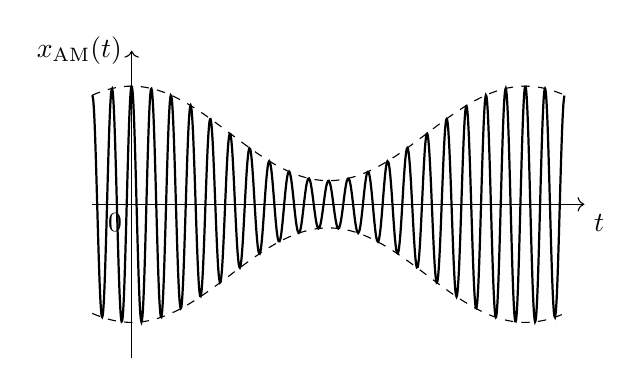
\begin{tikzpicture}[x=2.5cm, y=1.5cm]
      \draw[thin,->] (-0.2,0) -- (2.3,0) node[anchor=north west] {$t$};
      \draw[thin,->] (0,-1.3) -- (0,1.3) node[anchor=east] {$x_\text{AM}(t)$};
      \node[anchor=north east] at (0,0) {$0$};
      \draw[thick,smooth,samples=500,domain=-0.2:2.2,variable=\x] 
        plot ({\x},{(0.6+0.4*cos(0.05*3600*\x))*cos(3600*\x)});
      \draw[thin,dashed,smooth,samples=500,domain=-0.2:2.2,variable=\x] 
        plot ({\x},{(0.6+0.4*cos(0.05*3600*\x))});
      \draw[thin,dashed,smooth,samples=500,domain=-0.2:2.2,variable=\x] 
        plot ({\x},{-(0.6+0.4*cos(0.05*3600*\x))});
    \end{tikzpicture}
    \caption{\label{fig:AM}
      Amplitude modulation according to \cref{eqn:AM} with $a_C=0.6$, $a_M=0.4$,
      $x_C(t) = \cos(2\pi ft)$, and $x_M(t) = \cos\!\big(2\pi(0.05f)t\big)$}
  \end{subfigure}\hfill
  \begin{subfigure}[t]{0.47\textwidth}
    \centering
    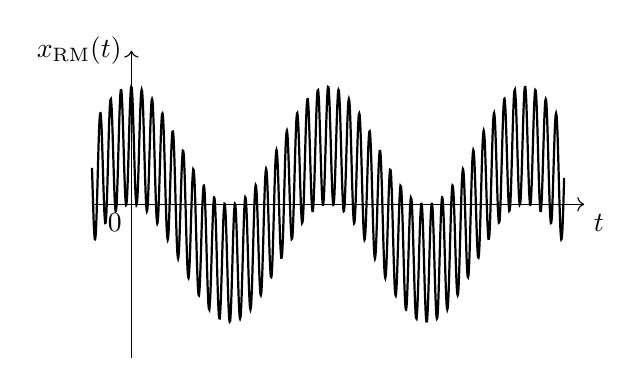
\begin{tikzpicture}[x=2.5cm, y=1.5cm]
      \draw[thin,->] (-0.2,0) -- (2.3,0) node[anchor=north west] {$t$};
      \draw[thin,->] (0,-1.3) -- (0,1.3) node[anchor=east] {$x_\text{RM}(t)$};
      \node[anchor=north east] at (0,0) {$0$};
      \draw[thick,smooth,samples=500,domain=-0.2:2.2,variable=\x] 
        plot ({\x},{cos(0.9*3600*\x)*cos(3600*\x)});
    \end{tikzpicture}
    \caption{\label{fig:RM}
      Ring modulation according to \cref{eqn:RM} with $x_C(t) = \cos(2\pi ft)$
      and $x_M(t) = \cos\!\big(2\pi(0.9f)t\big)$\newline~}
  \end{subfigure}
  \caption{\label{fig:AMRM}
    Examples of amplitude and ring modulation of two cosine waveforms}
\end{figure*}

\subsubsection{Phase and Frequency Modulation}
\label{sssec:FMPM}
For phase and frequency modulation we restrict the carrier signal to be a 
waveform
\begin{equation}
  \label{eqn:cwave}
  x_C(t) = \wf_C(2\pi ft),
\end{equation}
where we chose $\alpha=2\pi ft$ as the angle argument. \emph{Phase modulation}
is modifying the phase angle of the carrier waveform by a time-varying phase
shift signal $\varphi(t)$
\begin{equation}
  \notag
  x_\text{PM}(t)
  = w_C\big(2\pi ft + \varphi(t)\big).
\end{equation}
If whe choose another waveform, $w_M$, with a \emph{different} frequency $f_M$
and amplified by a gain factor $2\pi a_M$ as the phase shift signal
\begin{equation}
  \notag
  \varphi(t):=2\pi a_M\,w_M(2\pi f_Mt),
\end{equation}
we obtain a phase-modulated signal
\begin{equation}
  \label{eqn:PM}
  x_\text{PM}(t)
  = w_C\big(2\pi ft + 2\pi a_M\,w_M(2\pi f_M t)\big).
\end{equation}

For the following considerations we note, that the angle argument $2\pi f t$ of
the carrier waveform (\ref{eqn:cwave}) is a time-varying or, in other words, a
phase \emph{signal}
\begin{equation}
  \label{eqn:tvp}
  \varphi(t) = 2\pi f t.
\end{equation}
Actually, it is a linear function of time $t$ with a frequency-dependent slope 
$2\pi f$ an zero offset. Hence we can write the carrier waveform as
\begin{equation}
  \label{eqn:cwavep}
  x_C(t) = w_C\big(\varphi(t)\big)
  \quad\text{with } \varphi(t) = 2\pi f t.
\end{equation}
By definition, frequency is proportional to the time derivative of phase
\begin{equation}
  \label{eqn:tvf}
  f(t) = \frac{1}{2\pi}\,\frac{\d\,\varphi(t)}{\d\,t}.
\end{equation}
In general, also frequency may be time-varying, i.e., a frequency
\emph{signal}. The values of frequency signals according to \cref{eqn:tvf}
are called instantaneuos frequencies. Resolving \cref{eqn:tvf} for $\varphi(t)$
yields
\begin{equation}
  \varphi(t) = 2\pi\int\limits_0^t f(\tau)\,\tau + \varphi_0,
\end{equation} 
where $\tau$ denotes an auxiliary time variable---which is only needed because
$t$ is the upper limit of the integral---and $\varphi_0$ denotes an integration
constant which we will ignore in the following.

The concept of instantaneous frequencies generalizes the fixed frequencies we
used so far for our waveforms. We can see this easily by applying \cref{eqn:tvf} 
to \cref{eqn:tvp}:
\begin{equation}
  \notag
  f(t)
  = \frac{1}{2\pi}\,\frac{\d\,\varphi_C(t)}{\d\,t}
  = \frac{1}{2\pi}\,\frac{\d\left(2\pi ft\right)}{\d\,t}
  = f.
\end{equation}
\emph{Frequency modulation} is characterized by a time-varying frequency of the
carrier waveform
\begin{equation}
  \label{eqn:instfreq}
  f(t) = f+f_M(t)
\end{equation}
which is the sum of the constant tone frequency $f$ and a time-varying frequency
shift $f_M(t)$. Again, we choose another waveform, $w_M$, with a
\emph{different} frequency $f_M$ and amplified by a gain factor $2\pi a_M$ as
the modulating signal
\begin{equation}
  \notag
  f_M(t):=a_M\,w_M(2\pi f_M t)
\end{equation}
and obtain
\begin{equation}
  \label{eqn:FMtvf}
  f(t) = f + a_M\,w_M(2\pi f_M t)
\end{equation}
as instantaneous frequency of our carrier signal. Integrating \cref{eqn:FMtvf}
yields the respective phase signal
\begin{equation}
  \varphi(t) 
  = 2\pi \int\limits_0^t f(\tau)\,\d\tau
  = 2\pi f t + 2\pi\, a_M \int\limits_0^t w_M(2\pi f_M \tau)\,\d\tau
\end{equation} 
which we can introduce into \cref{eqn:cwavep} to obtain a formula for a
frequency-modulated waveform:
\begin{equation}
  \label{eqn:FM}
  x_{FM}(t) = w_C\!\!\left(2\pi f t + 2\pi\, a_M \int\limits_0^t w_M(2\pi f_M \tau)\,\d\tau\right)\!\!.
\end{equation}
%
Let's finally compare \cref{eqn:PM,eqn:FM}. We see that phase and frequency
modulation are closely related. Frequency modulation is actually just a phase
modulation with the integral over the modulating signal. For this reason, many
``FM'' synthesizers actually perform a phase modulation, as the latter is much
easier to implement and ``real'' FM introduces---by integrating over the
modulating signal---undesirable changes of the timbre with note frequency
\TODO{\cite{}}.

\cref{fig:PMFM} shows simple examples of phase and frequency modulation.
%
\workOn
%
\begin{figure*}[h]
  \centering
  \begin{subfigure}[t]{0.48\textwidth}
    \centering
    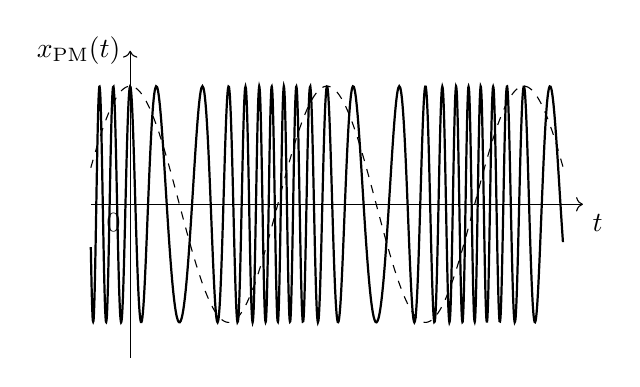
\begin{tikzpicture}[x=2.5cm, y=1.5cm]
      \draw[thin,->] (-0.2,0) -- (2.3,0) node[anchor=north west] {$t$};
      \draw[thin,->] (0,-1.3) -- (0,1.3) node[anchor=east] {$x_\text{PM}(t)$};
      \node[anchor=north east] at (0,0) {$0$};
      \draw[dashed,smooth,samples=500,domain=-0.2:2.2,variable=\x] 
        plot ({\x},{cos(0.1*3600*\x)});
      \draw[thick,smooth,samples=500,domain=-0.2:2.2,variable=\x] 
        plot ({\x},{cos(3600*\x + 0.1*3600*cos(0.1*3600*\x))});
    \end{tikzpicture}
    \caption{\label{fig:PM}
      Phase modulation according to \cref{eqn:PM} with $w_C(t) = \cos(2\pi ft)$, 
      $w_M(t) = \cos\!\big(2\pi(0.1f)t\big)$, and $a_M=0.1$}
  \end{subfigure}\hfill
  \begin{subfigure}[t]{0.48\textwidth}
    \centering
    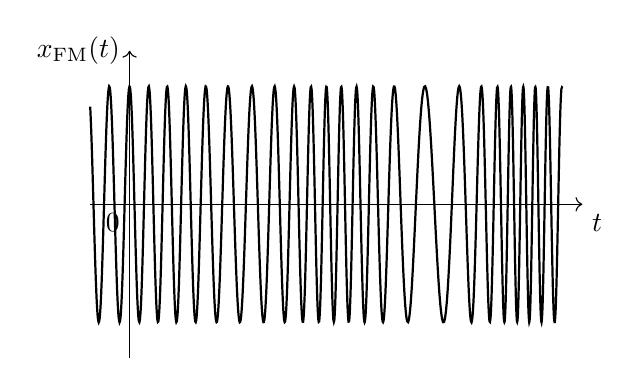
\begin{tikzpicture}[x=2.5cm, y=1.5cm]
      \draw[thin,->] (-0.2,0) -- (2.3,0) node[anchor=north west] {$t$};
      \draw[thin,->] (0,-1.3) -- (0,1.3) node[anchor=east] {$x_\text{FM}(t)$};
      \node[anchor=north east] at (0,0) {$0$};
      \draw[thick,smooth,samples=500,domain=-0.2:2.2,variable=\x] 
        plot ({\x},{cos((3600+0.05*3600*sin(0.1*3600*\x))*\x)});
%      \draw[thin,dashed,smooth,samples=500,domain=-0.2:2.2,variable=\x] 
%        plot ({\x},{(0.6+0.4*cos(0.05*3600*\x))});
%      \draw[thin,dashed,smooth,samples=500,domain=-0.2:2.2,variable=\x] 
%        plot ({\x},{-(0.6+0.4*cos(0.05*3600*\x))});
    \end{tikzpicture}
    \caption{\label{fig:FM}\workOn
      Frequency modulation according to \cref{eqn:FM} with $a_C=0.6$, $a_M=0.4$,
      $x_C(t) = \cos(2\pi ft)$, and $x_M(t) = \cos\!\big(2\pi\,(0.05f)\,t\big)$,
      i.e., $f_M=0.05\,f_C$\workOff}
  \end{subfigure}
  \caption{\label{fig:PMFM}
    Examples of phase and frequency modulation of two cosine waveforms}
\end{figure*}
%
\workOff

\subsubsection{Phase Distortion Modulation}
% Macros for drawing PD characteristic curve -->
\newcommand\PDMcharact[3]{{%
  \begin{scope}[shift={(#1,#2)}]
    \def\aI{#3}
    \def\xxI{1/(2*\aI)}
    \draw[thick,domain=0:\xxI,variable=\x] plot ({\x},{\a*\x});
    \draw[thick,domain=\xxI:1,variable=\x] plot ({\x},{(\a*\x+\a-1)/(2*\a-1)});
  \end{scope}
}}
\newcommand\PDMsine[3]{{%
  \begin{scope}[shift={(#1,#2)}]
    \def\aI{#3}
    \def\xxI{1/(2*\aI)}
    \draw[very thin,dashed,domain=0:1,variable=\x] plot ({\x},{0.5*sin(360*\x+90)});
    \draw[thick,domain=0:\xxI,variable=\x] plot ({\x},{0.5*sin(360*\a*\x+90)});
    \draw[thick,domain=\xxI:1,variable=\x] plot ({\x},{0.5*sin(360*((\a*\x+\a-1)/(2*\a-1))+90)});
  \end{scope}
}}
% <--
Phase distortion modulation (PDM) was invented in the early 1980's by \person{I.
Tomita}, \person{Y. Takahashi} and collegues of Casio Computer Ltd. for the CZ
music synthesizer series \cite{Ger09}. \cref{fig:PDMCzExample} shows an example
from the CZ manual. The VZ series uses waveform oscillators based on PDM.

Core element of PDM is a phase distortion characteristic curve as shown in
\cref{fig:PDMcc} \cite[p.\,20--21]{CZ1manual}.
%
\begin{figure*}[h!]
  \centering
  \begin{subfigure}[t]{0.3\textwidth}
    %\centering
    \hspace*{-28pt}
    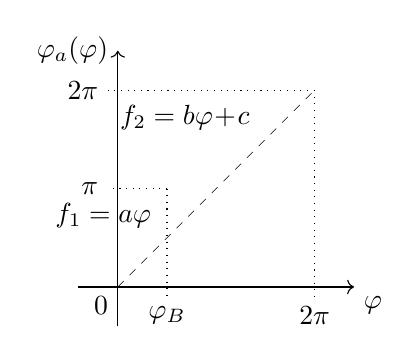
\begin{tikzpicture}[x=2.5cm, y=2.5cm]
      \def\a{2}; % a_min = 1; a_max = 2+sqrt(3) = 3.7321
      \def\xx{1/(2*\a)};
      %
      \draw[thin,->] (-0.2,0) -- (1.2,0) node[anchor=north west] {$\varphi$};
      \draw[thin,->] (0,-0.2) -- (0,1.2) node[anchor=east] {$\varphi_a(\varphi)$};
      \node[anchor=north east] at (0,0) {$0$};
      %
      \draw[very thin,dashed] (0,0) -- (1,1);
      \PDMcharact{0}{0}{\a};
      \node[anchor=south east] at({\xx/2},0.25) {$f_1=a\varphi$\!\!\!\!};
      \node[anchor=south east] at({\xx+(1-\xx)/2},0.75) {$f_2=b\varphi\!+\!c$\!\!\!\!};
      %
      \draw[thin,dotted] ({\xx},0.5) -- ({\xx}  ,-0.05) node[below] {$\varphi_B$};
      \draw[thin,dotted] (1    ,1  ) -- ( 1     ,-0.05) node[below] {$2\pi$};
      \draw[thin,dotted] ({\xx},0.5) -- (-0.05  , 0.5 ) node[left] {$\pi$};
      \draw[thin,dotted] (1    ,1  ) -- (-0.05  , 1   ) node[left] {$2\pi$};
    \end{tikzpicture}
    \caption{Piecewise linear phase\newline charateristics\label{fig:PDMcc}}
  \end{subfigure}
  \begin{subfigure}[t]{0.3\textwidth}
    %\centering
    \hspace*{-28pt}
    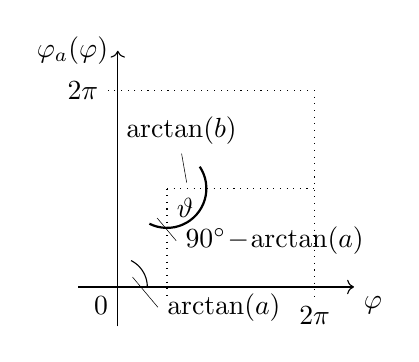
\begin{tikzpicture}[x=2.5cm, y=2.5cm]
      \def\a{2}; % a_min = 1; a_max = 2+sqrt(3) = 3.7321
      \def\b{\a/(2*\a-1)}
      \def\xx{1/(2*\a)};
      %
      \draw[thin,->] (-0.2,0) -- (1.2,0) node[anchor=north west] {$\varphi$};
      \draw[thin,->] (0,-0.2) -- (0,1.2) node[anchor=east] {$\varphi_a(\varphi)$};
      \node[anchor=north east] at (0,0) {$0$};
      %
      \draw[domain=0:{atan(\a)},variable=\x] plot ({0.15*cos(\x)}, {0.15*sin(\x)});
      \draw[very thin] (0.075,0.05) -- +(-50:0.2) node[right] {$\arctan(a)$};
      \draw[thick,domain={atan(\a)-180}:{atan(\b)},variable=\x] plot ({\xx+0.2*cos(\x)}, {0.5+0.2*sin(\x)});
      \node[anchor=north west] at ({\xx},0.5) {$\vartheta$};
      \draw[very thin] ({\xx-0.05},0.35) -- +( -50:0.15) node[right] {$90^{\circ}\!-\!\arctan(a)$};
      \draw[very thin] ({\xx+0.1 },0.53) -- +( 100:0.15) node[above] {$\arctan(b)$};
      \PDMcharact{0}{0}{\a};
      %
      \draw[thin,dotted] ({\xx},0.5) -- ({\xx},-0.05);
      \draw[thin,dotted] ({\xx},0.5) -- (1    , 0.5 );
      \draw[thin,dotted] (1    ,1  ) -- (1    ,-0.05) node[below] {$2\pi$};
      \draw[thin,dotted] (1    ,1  ) -- (-0.05, 1   ) node[left]  {$2\pi$};
    \end{tikzpicture}
    \caption{Distortion angle $\vartheta$,\newline $135^\circ\leq\vartheta\leq 180^\circ$\label{fig:PDMcc2}}
  \end{subfigure}
  \begin{subfigure}[t]{0.3\textwidth}
    %\centering
    \hspace*{-28pt}
    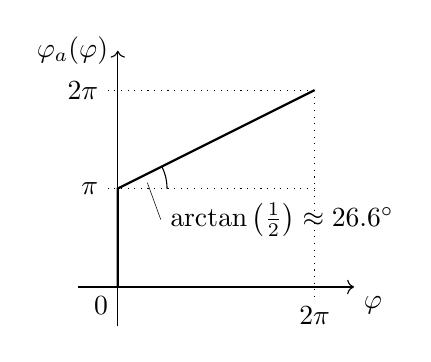
\begin{tikzpicture}[x=2.5cm, y=2.5cm]
      \draw[thin,->] (-0.2,0) -- (1.2,0) node[anchor=north west] {$\varphi$};
      \draw[thin,->] (0,-0.2) -- (0,1.2) node[anchor=east] {$\varphi_a(\varphi)$};
      \node[anchor=north east] at (0,0) {$0$};
      \draw[thick] (0,0) -- (0,0.5) -- (1,1);
      \draw[domain=0:{atan(0.5)},variable=\x] plot ({0.25*cos(\x)}, {0.5+0.25*sin(\x)});
      \draw[very thin] (0.15,0.53) -- +(-70:0.2) node[right] 
        {$\arctan\left(\frac{1}{2}\right)\approx 26.6^\circ$};
      \draw[thin,dotted] (1,1  ) -- (1    ,-0.05) node[below] {$2\pi$};
      \draw[thin,dotted] (1,1  ) -- (-0.05, 1   ) node[left]  {$2\pi$};
      \draw[thin,dotted] (1,0.5) -- (-0.05, 0.5 ) node[left]  {$\pi$};
    \end{tikzpicture}
    \caption{Minimum distortion angle\newline 
      $\vartheta_{\min}\approx 116.6\,^\circ$, $a\to\infty$\label{fig:PDMcc3}}
  \end{subfigure}
  \caption{Characteristic curve of phase distortortion}
\end{figure*}
We see that the curve consists of two straight sections
\begin{alignat}{5}
  f_1(\varphi) &= a\varphi, 
  & \quad 0&\leq\varphi <\varphi_B, 
  && \quad\text{connecting points } (0,0) \text{ and } (\varphi_B,\pi),\text{ and}
\\
  f_2(\varphi) &= b\varphi+c, 
  & \quad \varphi_B&\leq\varphi < 2\pi, 
  && \quad\text{connecting points } (\varphi_B,\pi) \text{ and } (2\pi,2\pi).
\end{alignat}
The slope $a$ of the first section is variable and can take real values $\geq
1$. The start and end points of the sections define the following constraints
\begin{alignat}{3}
  \label{eqn:PDMccc1}
  f_1(\varphi_B) &= a\varphi_B = \pi
  && \quad\leadsto \varphi_B = \frac{\pi}{a}
\\
  \label{eqn:PDMccc2}
  f_2(\varphi_B) &= \frac{\pi}{a}b + c = \pi
\\
  \label{eqn:PDMccc3}
  f_2(2\pi) &= 2\pi b + c = 2\pi
\end{alignat}
From \cref{eqn:PDMccc1,eqn:PDMccc2,eqn:PDMccc3} follows
\begin{equation}
  b = \frac{a}{2a-1}
  \quad\text{and}\quad
  c = \frac{2a-2}{2a-1}\pi,
\end{equation}
and finally
\begin{equation}
  \label{eqn:PDMcc}
  \varphi_a(\varphi)
  = \begin{cases}
      a\varphi
      & \text{for }0\leq\varphi < \frac{\pi}{a}
    \\[6pt]
      \dfrac{a\varphi+2\pi(a-1)}{2a-1}
      & \text{for }\frac{\pi}{a}\leq\varphi < 2\pi 
    \end{cases}
  \text{ with }a\geq 1
  \qquad\text{\ML\TT{phipd=vVZtools.PDMcc(phi,a)}.}
\end{equation}

\REMARK{An alternate phase distortion characteristic $f_a(x)$ with domain $0\leq
x < 1$ taking values $0\leq f_a(x) < 1$ may be needed for Reaktor
implementation:
\begin{equation}
  f_a(x) = 
  \begin{cases}
    ax                   & 0\leq x < \frac{1}{2a}\\
    \dfrac{ax+a-1}{2a-1} & \frac{1}{2a} \leq x< 1
  \end{cases}
  \qquad\text{with }a\geq 1.
\end{equation}}

\noindent
Modulation depth can also be expressed by the angle between the straight
sections
\begin{align}
  \notag
  \vartheta 
  &= \pi-\arctan(a)+\arctan(b)
\\
  \label{eqn:PDMaToTheta}
  &= \pi-\arctan(a)+\arctan\!\left(\frac{a}{2a-1}\right)
  \qquad\qquad\text{\ML\TT{theta=vVZtools.pdmA2theta(a)}}
\end{align}
measured in degrees (see \cref{fig:PDMcc2}). Literature states that the
permissible range is $135^\circ\leq\vartheta\leq 180^\circ$ \cite{Ger09}.
However, for the wavetable of the VZ series this restriction does not seem to
hold. Measurement yielded angles down to $123^\circ$ corresponding to slope
parameters $a>10$.\footnote{see
\TT{matlab/PhaseDistortionModulationAnalysis.mlx}} As I did not manage to solve
\cref{eqn:PDMaToTheta} for $a$, I just plot the function and print a lookup
table in \cref{fig:PDMaToTheta}.
%
\begin{figure*}
  \centering
  \begin{subfigure}{0.45\textwidth}
    \centering
    \begin{tikzpicture}[x=1cm, y=2cm]
      \def\offset{-120};
      \def\scale{1/45};
      \draw[thin,->] (-0.4,0) -- (5,0) node[anchor=north west] {$a$};
      \draw[thin,->] (0,-0.2) -- (0,1.5) node[anchor=east] {$\vartheta/^{\circ}$};
      \draw[thick,domain=1:5,variable=\x] plot ({\x},{(180-atan(\x)+atan(\x/(2*\x-1))+\offset)*\scale});
      \draw[thin,dotted] (1,{(180+\offset)*\scale}) -- (-0.2,{(180+\offset)*\scale}) node[left] {$180$}; 
      \draw[thin,dotted] (1,{(180+\offset)*\scale}) -- (1,-0.1) node[below] {$1$}; 
      \draw[thin,dotted] (3.73,{(135+\offset)*\scale}) -- (-0.2,{(135+\offset)*\scale}) node[left] {$135$}; 
      \draw[thin,dotted] (3.73,{(135+\offset)*\scale}) -- (3.73,-0.1) node[below] {$2\!+\!\sqrt{3}$}; 
    \end{tikzpicture}
    \caption{Distortion angle parameter $\vartheta$ as a function of slope parameter $a$}
  \end{subfigure}
  \begin{subfigure}{0.45\textwidth}
    \centering\vspace*{-3pt}
    \begin{tabular}{llcll}\toprule
      $\vartheta/^\circ$ & $a$ & & $\vartheta/^\circ$ & $a$    \\\midrule
      $116.6$ & $\infty$                     && $150$ & $2.02$ \\
      $120$   & $20.07$                      && $155$ & $1.74$ \\
      $125$   & $8.19$                       && $160$ & $1.52$ \\
      $130$   & $5.14$                       && $165$ & $1.35$ \\
      $135$   & $2\!+\!\sqrt{3}\approx 3.73$ && $170$ & $1.21$ \\
      $140$   & $2.92$                       && $175$ & $1.10$ \\
      $145$   & $2.39$                       && $180$ & $1.00$ \\\bottomrule
    \end{tabular}
    \caption{Lookup table}
  \end{subfigure}
  \caption{Relation between distortion angle parameter $\vartheta$ and slope
  parameter $a$, see \cref{eqn:PDMaToTheta}\label{fig:PDMaToTheta}}
\end{figure*}

\begin{figure*}
  \hspace*{37pt}
  \begin{subfigure}{0.33\textwidth}
    \hspace*{-37pt}
    \scalebox{0.65}{
      \begin{tikzpicture}[x=2cm, y=2cm]
        \def\a{1}; % a_min = 1; a_max = 2+sqrt(3) = 3.7321
        \def\xx{1/(2*\a)};
        %
        \draw[thin,->] (-0.2,0) -- (2.3,0) node[anchor=north west] {$\varphi$};
        \draw[thin,->] (0,-0.2) -- (0,1.3) node[anchor=east] {$\varphi_a(\varphi)$};
        \node[anchor=north east] at (0,0) {$0$};
        \draw[thin,->] (-0.2,-1) -- (2.3,-1) node[anchor=north west] {$\varphi$};
        \draw[thin,->] (0,-1.7) -- (0,-0.3) node[anchor=east] {$\cos\!\big(\varphi_a(\varphi)\big)$};
        %
        \PDMcharact{0}{0}{\a};
        \PDMcharact{1}{0}{\a};
        \PDMsine{0}{-1}{\a};
        \PDMsine{1}{-1}{\a};
        %
        \draw[thin] (0.05,-0.5) -- (-0.05,-0.5) node[left] {$1$};
        \draw[thin] (0.05,-1.5) -- (-0.05,-1.5) node[left] {$-1$};
        \node[anchor=north west] at (1,0) {\!$2\pi$};
        \node[anchor=north west] at (2,0) {\!$4\pi$};
        \draw[thin,dotted] ({\xx}  ,0.5) -- ({\xx}  ,-1.5);
        \draw[thin,dotted] ({1+\xx},0.5) -- ({1+\xx},-1.5);
        \draw[thin,dotted] (1      ,1  ) -- ( 1     ,-0.5);
        \draw[thin,dotted] ({1+\xx},0.5) -- (-0.05  , 0.5 ) node[left] {$\pi$};
        \draw[thin,dotted] (2      ,1  ) -- (-0.05  , 1   ) node[left] {$2\pi$};
        \draw[thin,dotted] (2      ,1  ) -- ( 2     ,-0.5);
      \end{tikzpicture}
    }
    \caption{$\vartheta=180^\circ$ ($a=1$)\newline no modulation\newline ~}
  \end{subfigure}%\hspace*{-3pt}
  \begin{subfigure}{0.33\textwidth}
    \hspace*{-37pt}
    \scalebox{0.65}{
      \begin{tikzpicture}[x=2cm, y=2cm]
        \def\a{2}; % a_min = 1; a_max = 2+sqrt(3) = 3.7321
        \def\xx{1/(2*\a)};
        %
        \draw[thin,->] (-0.2,0) -- (2.3,0) node[anchor=north west] {$\varphi$};
        \draw[thin,->] (0,-0.2) -- (0,1.3) node[anchor=east] {$\varphi_a(\varphi)$};
        \node[anchor=north east] at (0,0) {$0$};
        \draw[thin,->] (-0.2,-1) -- (2.3,-1) node[anchor=north west] {$\varphi$};
        \draw[thin,->] (0,-1.7) -- (0,-0.3) node[anchor=east] {$\cos\!\big(\varphi_a(\varphi)\big)$};
        %
        \draw[very thin,dashed] (0,0) -- (1,1);
        \draw[very thin,dashed] (1,0) -- (2,1);
        \PDMcharact{0}{0}{\a};
        \PDMcharact{1}{0}{\a};
        \PDMsine{0}{-1}{\a};
        \PDMsine{1}{-1}{\a};
        %
        \draw[thin] (0.05,-0.5) -- (-0.05,-0.5) node[left] {$1$};
        \draw[thin] (0.05,-1.5) -- (-0.05,-1.5) node[left] {$-1$};
        \node[anchor=north west] at (1,0) {\!$2\pi$};
        \node[anchor=north west] at (2,0) {\!$4\pi$};
        \draw[thin,dotted] ({\xx}  ,0.5) -- ({\xx}  ,-1.5);
        \draw[thin,dotted] ({1+\xx},0.5) -- ({1+\xx},-1.5);
        \draw[thin,dotted] (1      ,1  ) -- ( 1     ,-0.5);
        \draw[thin,dotted] ({1+\xx},0.5) -- (-0.05  , 0.5 ) node[left] {$\pi$};
        \draw[thin,dotted] (2      ,1  ) -- (-0.05  , 1   ) node[left] {$2\pi$};
        \draw[thin,dotted] (2      ,1  ) -- ( 2     ,-0.5);
      \end{tikzpicture}
    }
    \caption{$\vartheta=150^\circ$ ($a\approx 2$)~~~~~~~~~~~~~~~~~~~\newline ~\newline ~}
  \end{subfigure}%\hspace*{-3pt}
  \begin{subfigure}{0.33\textwidth}
    \hspace*{-37pt}
    \scalebox{0.65}{
      \begin{tikzpicture}[x=2cm, y=2cm]
        \def\a{3.73}; % a_min = 1; a_max = 2+sqrt(3) = 3.7321
        \def\xx{1/(2*\a)};
        %
        \draw[thin,->] (-0.2,0) -- (2.3,0) node[anchor=north west] {$\varphi$};
        \draw[thin,->] (0,-0.2) -- (0,1.3) node[anchor=east] {$\varphi_a(\varphi)$};
        \node[anchor=north east] at (0,0) {$0$};
        \draw[thin,->] (-0.2,-1) -- (2.3,-1) node[anchor=north west] {$\varphi$};
        \draw[thin,->] (0,-1.7) -- (0,-0.3) node[anchor=east] {$\cos\!\big(\varphi_a(\varphi)\big)$};
        %
        \draw[very thin,dashed] (0,0) -- (1,1);
        \draw[very thin,dashed] (1,0) -- (2,1);
        \PDMcharact{0}{0}{\a};
        \PDMcharact{1}{0}{\a};
        \PDMsine{0}{-1}{\a};
        \PDMsine{1}{-1}{\a};
        %
        \draw[thin] (0.05,-0.5) -- (-0.05,-0.5) node[left] {$1$};
        \draw[thin] (0.05,-1.5) -- (-0.05,-1.5) node[left] {$-1$};
        \node[anchor=north west] at (1,0) {\!$2\pi$};
        \node[anchor=north west] at (2,0) {\!$4\pi$};
        \draw[thin,dotted] ({\xx}  ,0.5) -- ({\xx}  ,-1.5);
        \draw[thin,dotted] ({1+\xx},0.5) -- ({1+\xx},-1.5);
        \draw[thin,dotted] (1      ,1  ) -- ( 1     ,-0.5);
        \draw[thin,dotted] ({1+\xx},0.5) -- (-0.05  , 0.5 ) node[left] {$\pi$};
        \draw[thin,dotted] (2      ,1  ) -- (-0.05  , 1   ) node[left] {$2\pi$};
        \draw[thin,dotted] (2      ,1  ) -- ( 2     ,-0.5);
      \end{tikzpicture}
    }
    \caption{$\vartheta=135^\circ$ ($a\approx 3.73$)\newline resembling a sawtooth\newline signal}
  \end{subfigure}
  \caption{Example of phase distortion modulation of a cosine adapted from
    \cite[p.\,20--21, Figs.\,1--3]{CZ1manual}\label{fig:PDMCzExample}. Phase
    angles $\varphi<0$ and $\varphi\geq 2\pi$ are wrapped into the base interval
    $0 \leq \varphi <2 \pi.$ Note that \cite{CZ1manual} uses
    $-\cos\!\big(\varphi\big)$ as carrier signal.}
\end{figure*}
Waveforms \TT{SINE} and \TT{SAW1}--\TT{SAW5} of VZ-1/VZ-10M resemble
phase-distorted cosine waves
\begin{equation}
  w(\varphi) = \cos\!\big(\varphi_a(\varphi)\big).
\end{equation}
\Cref{fig:PDMCzExample} shows some examples.

\subsubsection{Wavetable Osciallators}
The original VZ-1/VZ-10M is apparently based on wavetable oscillators
\cite[p.\,34]{VZ1Manual}. Such oscillators contain a set of digital waveforms,
each comprising exactly one signal period. Depending on the pitch, these
waveforms are played back at different rates. \TODO{\cref{fig:wavtab}} shows an
example of a VZ waveform (\TT{SAW4}).

Formally, a single waveform can be expressed by
\begin{equation}
  w(\varphi)\quad\text{with } 0\leq\varphi<2\pi,
\end{equation}
where the argument $\varphi$ is a phase angle. A oscillator based on this
waveform uses a time-varying phase angle $\varphi(t)$. Its output signal can be
written as
\begin{equation}
  \label{eqn:WavTabOsc}
  x(t) 
  = w\big(\varphi(t)\big)
  = w\big(2\pi (f_0t\!\!\!\mod 1)\big)\quad\text{with } -1\leq x(t)\leq 1
\end{equation}
where $w$ denotes a waveform, $f_0\in\mathbb{R}^{> 0}$ denotes the note
frequency in Hertz, and $t$ denotes the time in seconds. Further, we denote by
\begin{equation}
  x\!\!\!\mod 1 := x-\lfloor x\rfloor\quad\text{with } 0\leq (x\!\!\!\mod 1)<1
\end{equation}
the decimal fraction of the real valued quantity $x$. Hence, the argument
$\varphi(t) = 2\pi (f_0t\!\!\!\mod 1)$ on the right side of \cref{eqn:WavTabOsc}
involves resetting the phase angle of the waveform to zero whenever the cycle
length $2\pi$ is surpassed. \TODO{\cref{fig:WavTabOsc}} shows an example.

We will use the circuit symbol \TODO{\ldots} for a wavetable oscillator.

\subsection{VZ Hardware}
\subsubsection{Waveforms}
The VZ series features eight waveforms: sine (\TT{SINE}), five sawtooth-shaped
waveforms (\TT{SAW1}--\TT{SAW5}), white noise (\TT{NOISE1}), and a mixture of
white noise and a sine tone (\TT{NOISE2}). The \TT{SAWn} waveforms resemble
phase-distortion modulated cosines
\begin{equation}
  x(\varphi) 
  = \cos\big(\varphi_a(\varphi)\big)
  = \sin\!\left(\varphi_a(\varphi)+\frac{\pi}{2}\right)\!,
\end{equation} 
where $\varphi_a(\varphi)$ denotes the phase distortion characteristic according
to \cref{eqn:PDMcc} with slope parameter $a$. Thorough analysis of recordings
(see \TT{matlab/PhaseDistortionModulationAnalysis.mlx}) shows that VZ's actual
\TT{SAWn} waveforms exhibit phase shifts of the carrier signal and---even
worse---the measured phase distortion characteristics is \emph{not} pieceweise
linear. \TODO{\cref{fig:actualPDM}} shows an example. I conclude that VZ-1 does
\emph{not} employ PDM as described in \cite{CZ1manual} but some approximation of
it. Consequently, I have two options for the replica
\begin{itemize}
  \item purist: implement a PDM oscillator anyway or
  \item thruthful: implement a wave table oscillator using wave cycles sampled
        from the VZ-1.
\end{itemize}

\subsection{Replica}
\subsubsection{Voltage-Controlled Oscillators (VCO)}
\workOn
In order to read the wavetable out of my VZ-1, I proceeded as follows
\begin{enumerate}
  \item
    Set the master tune of VZ-1 to $440\,$Hz in \TT{MENU 3-00},
  \item
    Initialize a new voice,
  \item
    Mute all oscillator modules except \TT{M1} and configure line \TT{A} as 
    \TT{MIX} in \TT{MENU 1/00},
  \item 
    In \TT{MENU 1/02}, set \TT{M1} to a fix pitch of \TT{OCT=00}, \TT{NOTE=00},
    \TT{FINE=08} to generate tones with a frequency of $46^7\!/_8$\,Hz (see
    below),
  \item
    Configure all amplitude controls of \TT{M1} for maximum signal output and
    set a trivial amplitude envelope mimicking a mere gate signal,
  \item
    Disable all LFOs and MIDI controllers on \TT{M1}.
\end{enumerate} 
I recorded with the Komplete Audio 6 sound interface at a sampling frequency
of $f_S=48$\,kHz. Each waveform in the wavetable shall contain $K=1024$ samples
for one full cycle. Hence, the ``natural'' frequency of the waveforms---i.e., 
when reading out at $48$\,kSamples per second---is
\begin{equation}
  f_0 
  = \frac{f_A}{K} 
  = \frac{48000\,\text{Hz}}{1024}
  = 46^7\!/_8\,\text{Hz}
\end{equation}
which corresponds to the musical note F\#1 + $23$\,ct. Using the fix pitch
settings above, one cycle of the waveform being recorded is exactly $1024$
samples long and no resampling is necessary.
\workOff

\subsubsection{Voltage-Controlled Amplifiers (VCA)}

%%%%%%%%%%%%%%%%%%%%%%%%%%%%%%%%%%%%%%%%%%%%%%%%%%%%%%%%%%%%%%%%%%%%%%%%%%%%%%%

\section{Control Signal Generators}

%%%%%%%%%%%%%%%%%%%%%%%%%%%%%%%%%%%%%%%%%%%%%%%%%%%%%%%%%%%%%%%%%%%%%%%%%%%%%%%

\section{MIDI SysEx Control}
\ISSUE{Reaktor 6 does not seem to support MIDI SysEx. Circumvent by control
automation?}

%%%%%%%%%%%%%%%%%%%%%%%%%%%%%%%%%%%%%%%%%%%%%%%%%%%%%%%%%%%%%%%%%%%%%%%%%%%%%%%

\section{GUI Replica}
\workOn
\begin{itemize}
  \item LCD dot matrix display 96$\times$64 pixels
\end{itemize}
\workOff

%%%%%%%%%%%%%%%%%%%%%%%%%%%%%%%%%%%%%%%%%%%%%%%%%%%%%%%%%%%%%%%%%%%%%%%%%%%%%%%

%\pagebreak
\addcontentsline{toc}{section}{References}
\bibliographystyle{plain}
\bibliography{Casio-VZ-virtual-instrument}

\end{document}

%% EOF